\section{実験装置の改良による影響}
\label{sec:reexp}
先行研究\cite{ref:8}において,電磁石を用いて,磁力によって球の把持を行っていた.本研究において,強磁性体以外の球の把持を行うため,真空ポンプを用いて吸引する手法に変更した.その把持手法の変化に伴う影響を議論する.

\subsection{実験装置}

電磁石を用いた実験装置をFig.\ref{fig:magnet_device}に示す.電磁石の磁力によって落下球の把持を行った.球を落下させるとき,電磁石への通電を切り,落下方向に力を加えて球を落下させた.また,本実験は先行研究と同様の条件で行うため,外寸において高さ248.5mm,幅47mm,奥行き47mm,厚さ3.5mmの矩形ガラス水槽で実験を行った.また,照射する超音波の周波数は39kHzとした.

\begin{figure}[H]
    \centering
    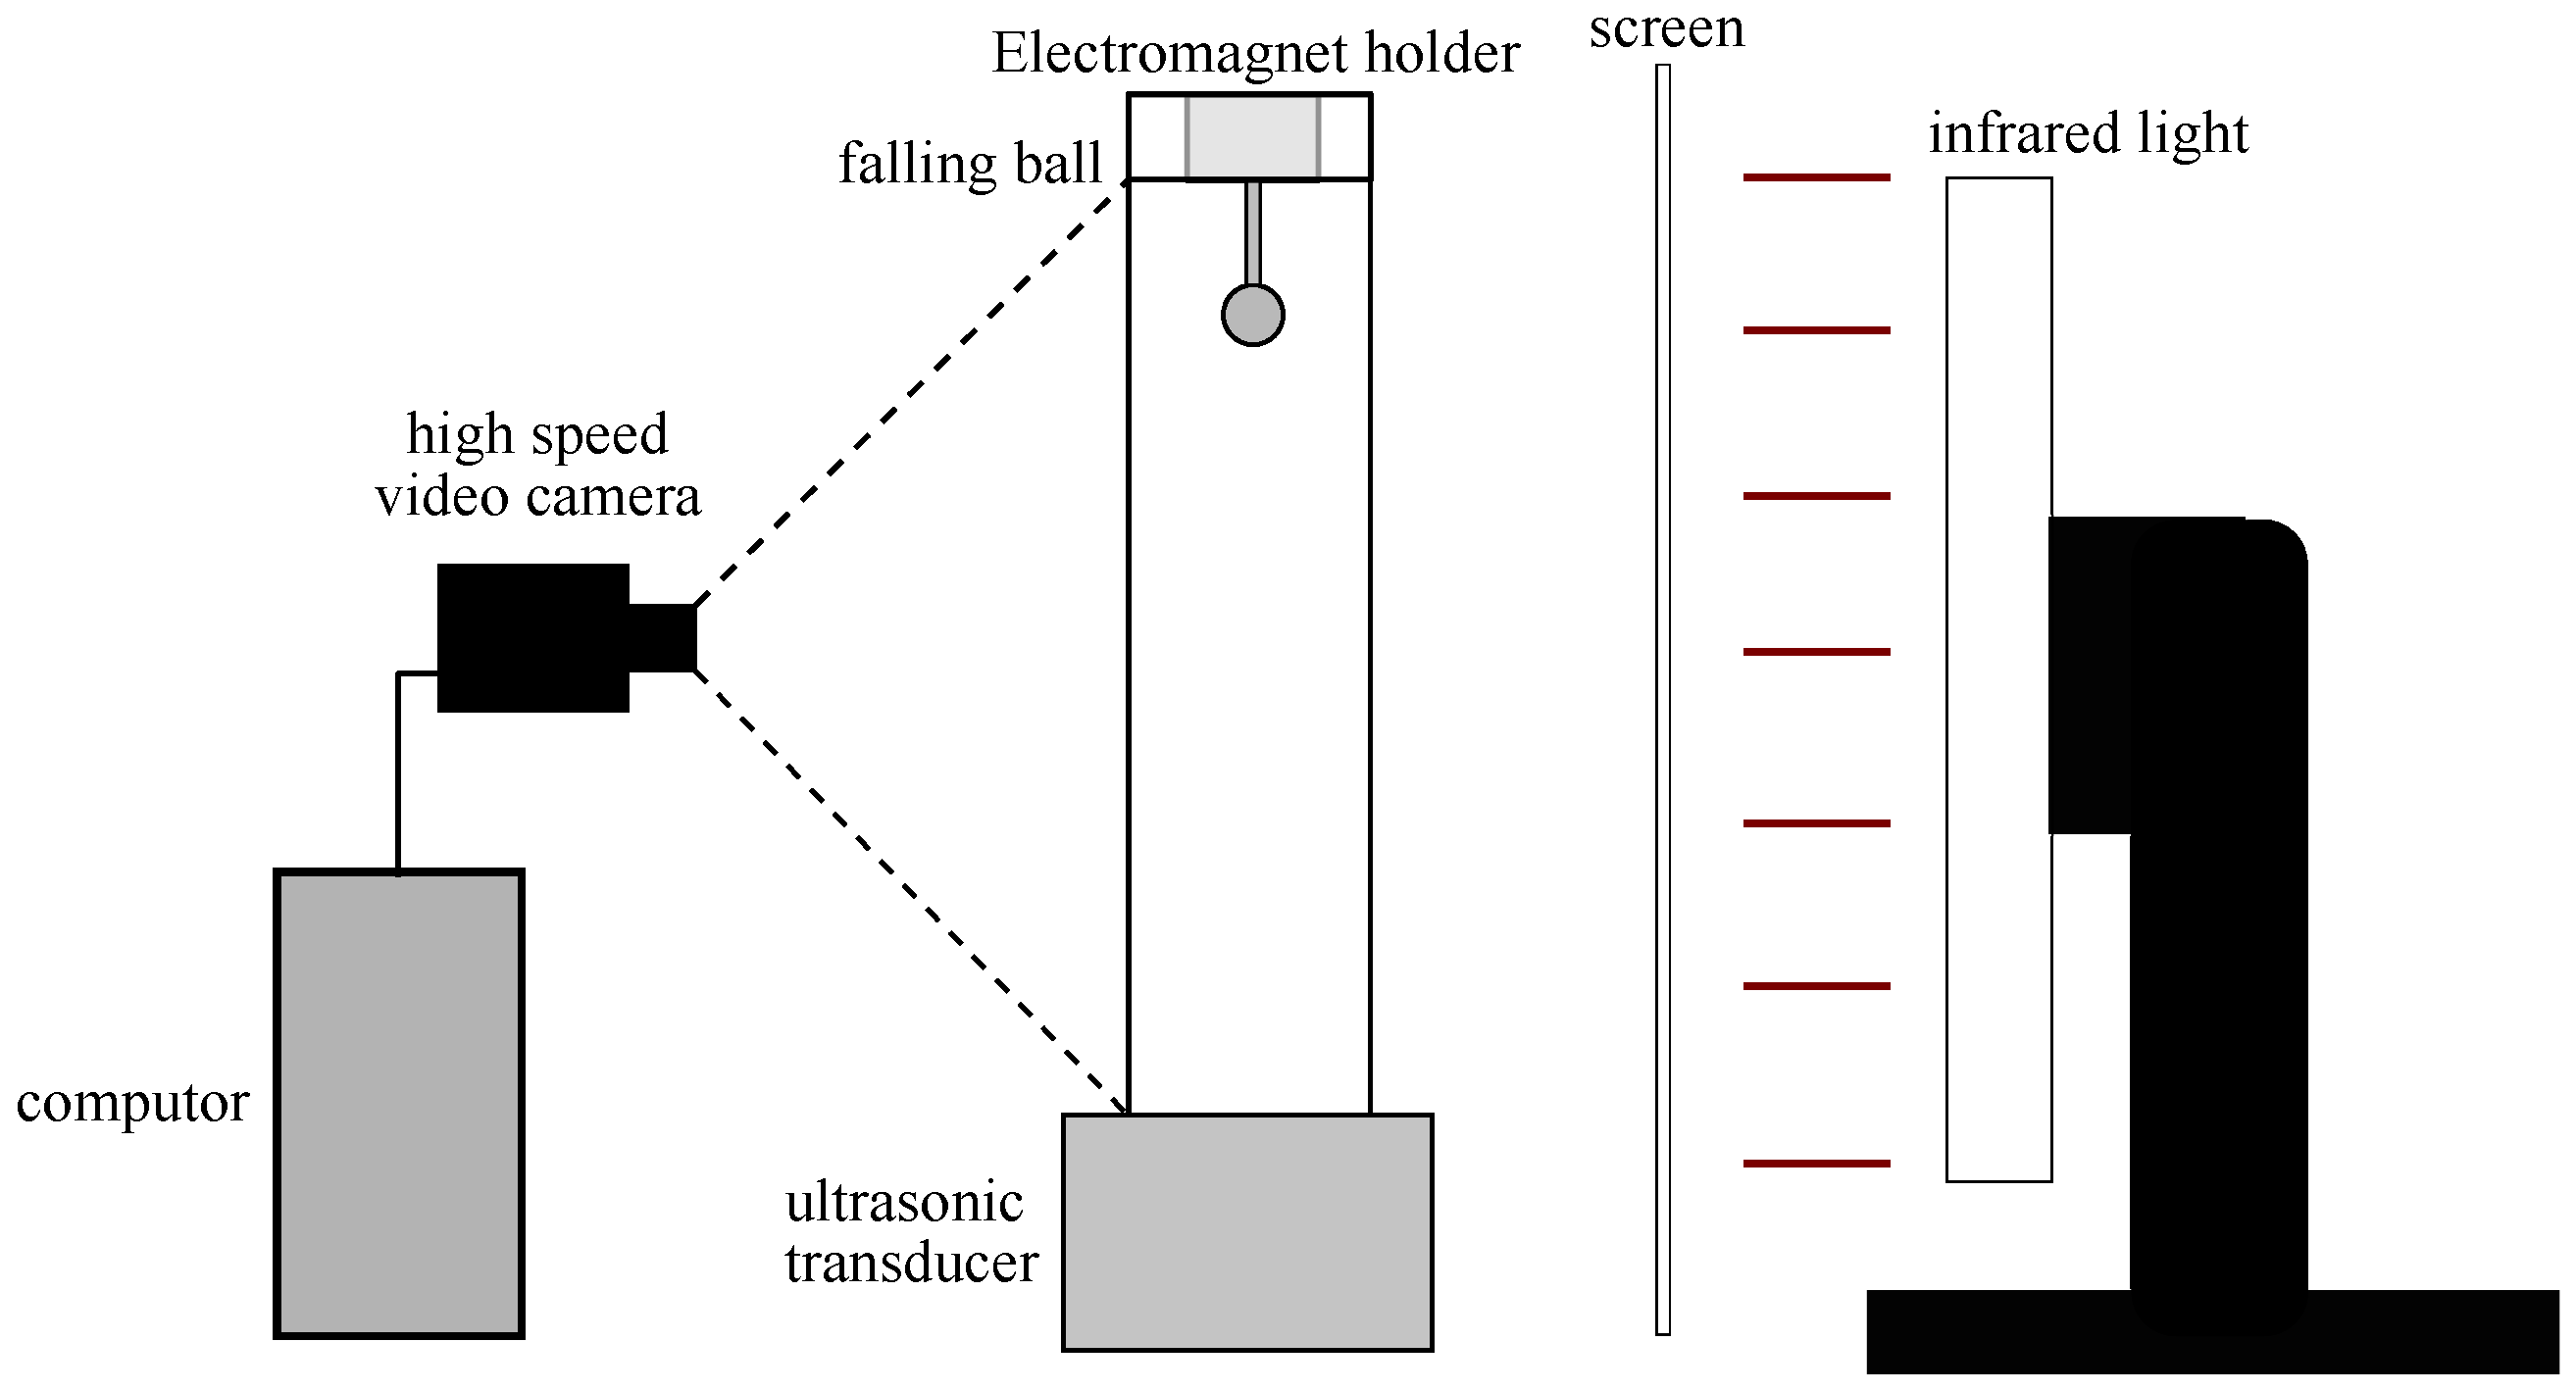
\includegraphics[width=0.95\textwidth]{X-Appendix/device/magnet_device.eps}
    \caption{Schematic view of the experimental apparatus by using electromagnet.}
    \label{fig:magnet_device}
\end{figure}

\subsection{落下実験結果}
真空ポンプを用いて球を把持した場合と電磁石を用いて球を把持した場合の結果をFig \ref{fig:falling-A}に示す.縦軸は落下速度,横軸は落下開始時からの経過時間である.落下開始時に電磁石を用いた場合はオーバーシュートが見られるが,真空ポンプを用いた場合はオーバーシュートが見られなかった.これは,落下開始時における初速による影響が考えられる.本研究\ref{sec:interval-velocity}章にて,初速を与えた場合に関して考える.

終端速度と高速化度合の関係をFig\ref{fig:falling-Udiff}(a)に示す.縦軸は高速化度合,横軸は落下球の終端速度である.真空ポンプを用いて球を把持した場合,先行研究である岩室\cite{ref:8}や電磁石を用いて球を把持した場合と比較し,超音波照射による高速化が顕著に現れなかった.また,粘度比と音響境界層を球の半径で規格化した値と高速化度合の関係をFig.\ref{fig:falling-Udiff}(b)に示す.真空ポンプを用いて把持した場合,粘度比と音響境界層を球の半径で規格化した値が0.1を超える領域に存在する.これは,本研究\ref{sec:viscosity}章で示した高速化があまり見られなくなる領域となっており,真空ポンプを用いて把持した場合,高速化があまり見られていない.先行研究である岩室\cite{ref:8}と今回の実験結果に差異が生じた理由は,作製した溶液の特性や音響圧の違いによって生じたと考えられる.
\begin{figure}[H]
    \centering
    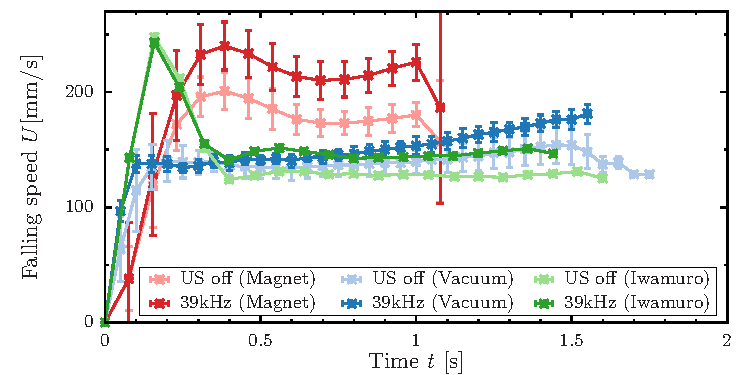
\includegraphics[width=1\textwidth]{./X-Appendix/magnet_vacuum/magnet_vacuum.eps}
    \caption{Falling speed of a sphere in 1.0wt.\%PAA solution with and without ultrasound irradiation.}
    \label{fig:falling-A}
\end{figure}

\begin{figure}[H]
    \centering
    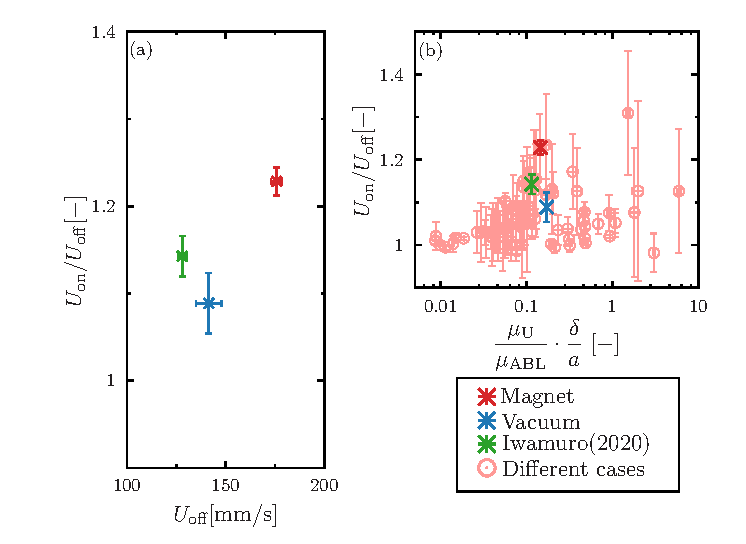
\includegraphics[width=1\textwidth]{./X-Appendix/magnet_vacuum/magnet_vacuum_cal.eps}
    \caption{Relationship velocity ratio and (a)terminal velocity, (b)viscosity ratio.}
    \label{fig:falling-Udiff}
\end{figure}

% \subsection{落下開始時のオーバーシュートへの影響}
% \label{sec:dis-de}

% 今回,球を把持する手法を,電磁石を用いて把持する方法から真空ポンプを用いて把持する方法に変化させた.この時,落下開始時0-0.3sにおける落下速度のオーバーシュートが,先行研究\cite{ref:8,ref:9}より小さくなった.落下開始時のオーバーシュートは弾性による影響によって生じる\cite{ref:12}.以下で,オーバーシュートが見られなくなった原因を,物質の流動性を表す$De$数より考える.$De$数が大きくなると,弾性的傾向が強くなり,$De$数が小さくなると,粘性的流動を表す.

% $De$数は下記の様に緩和時間$\lambda$,代表時間$T$の比で表される.
% \begin{equation}
%     De = \frac{\lambda}{T} .
%     \label{eq:De}
% \end{equation}
% 代表時間$T$に関して,超音波照射を行っていない場合の球の落下条件においても考えるため,
% \begin{equation}
%     T = \frac{a}{U} ,
%     \label{eq:T}
% \end{equation}
% となる.ここで,球の落下速度$U$,球の半径$a$である.また,緩和時間$\lambda$は,粘度$\mu$,貯蔵弾性率$G'$を用いて,
% \begin{equation}
%     \lambda \approx \frac{\mu}{G'} ,
%     \label{eq:lamda}
% \end{equation}
% と見積もられる.緩和時間は変形の経過時間において,粘弾性流体が流体的挙動を示すか,固体的挙動を示すかの指標である\cite{ref:sakanishi}.粘度$\mu$に関して,落下球によるせん断領域における粘度となるため,式(\ref{eq:muU})の$\mu_\text{U}$を用いる.

% これら式(\ref{eq:De}),(\ref{eq:T}),(\ref{eq:lamda}),(\ref{eq:muU})より,$De$数は,
% \begin{equation}
%     De \sim \frac{k}{G'} {\left(\frac{U}{a}\right)}^n ,
%     \label{eq:De2}
% \end{equation}
% となり,粘度定数$k$,貯蔵弾性率$G'$,落下速度$U$,球の半径$a$によって見積もられる.

% 貯蔵弾性率$G'$に関して,Fig.\ref{fig:PAA-elast}にて示した応力との関係性の結果を用いる.ここで応力$\tau$は,落下球によって生じた応力$\tau_\text{U}$を用いる.

% Fig. \ref{fig:iwamuro-fall}に先行研究であるIwamuro \textit{et al}.\cite{ref:8}の球径ごとの実験結果を示す.Fig.\ref{fig:falling-A}, \ref{fig:iwamuro-fall}それぞれの結果より,ピーク速度$U_{peak}$と終端速度$U_{ave}$を算出した.続いて,式(\ref{eq:tau-cal})を用いて,それぞれの速度における応力$\tau_{peak}$,$\tau_{ave}$の算出を行った.これら算出結果と先行研究の計測結果Fig.\ref{fig:iwamuro-G}より,貯蔵弾性率$G'$も求めた.これらの結果を,Table \ref{table:iwamuro}に示す.

% また,式(\ref{eq:muU})を用いて,ピーク速度/終端速度それぞれの粘度$\mu_{peak}$,$\mu_\text{U}$を概算した.これらの粘度を式(\ref{eq:lamda})に代入し,それぞれの緩和時間$\lambda_{peak}$,$\lambda_{ave}$の算出を行った.そして,それらの緩和時間より,式(\ref{eq:De})を用いて,それぞれの$De$数,$De_{peak}$,$De_{ave}$を求めた.これらの結果を,Table \ref{table:iwamuro2}に示す.

% Table \ref{table:iwamuro2}より,ピーク速度より求めた$De_{peak}$と,終端速度より求めた$De_{ave}$において,大きな差異が見られないことが分かった.以降,$De_{peak}$に関してのみ議論を行う.$De_{peak}$に関して,落下速度のオーバーシュート$U_{peak}/U_{ave}$との関係をFig.\ref{fig:De-overshoot}に示す.横軸は$De$数,縦軸は落下速度のオーバーシュート$U_{peak}/U_{ave}$である.この図より,$De$数とオーバーシュートには正の相関があり,$De$数が増加するとオーバーシュートも大きくなることが分かった.

% \begin{table}[H]
%     \caption{Peak speed $U_{peak}$/ terminal speed $U_{ave}$, stress $\tau$, storage modulus $G'$ Calculation result.}
%     \label{table:iwamuro}
%     \centering
%     \begin{tabular}{ccccccc}
%         \hline
%         \multirow{2}{*}{実験者}  & 球直径[mm] & ピーク速度[mm/s] & 終端速度[mm/s] & \multicolumn{2}{c}{応力[Pa]} & 貯蔵弾性率[Pa]        \\
%                                  & $D=2a$     & $U_{peak}$       & $U_{ave}$      & $\tau_{peak}$                & $\tau_{ave}$   & $G'$ \\
%         \hline \hline
%         \multirow{8}{*}{Iwamuro} & 3          & 10.08            & 9.05           & 14.6                         & 14.2           & 8    \\
%                                  & 4          & 23.2             & 19.4           & 16.5                         & 15.9           & 7    \\
%                                  & 5          & 34.8             & 32.6           & 17.2                         & 17.0           & 6.7  \\
%                                  & 6          & 46.3             & 54.8           & 17.6                         & 18.3           & 6.5  \\
%                                  & 7          & 79.8             & 82             & 19.3                         & 19.4           & 5.5  \\
%                                  & 8          & 130              & 113            & 20.9                         & 20.3           & 5    \\
%                                  & 9          & 193              & 133            & 22.3                         & 20.5           & 4    \\
%                                  & 10         & 256              & 168            & 23.2                         & 21.2           & 3.5  \\
%         \hline \hline
%         Niwa                     & 10         & 148              & 144            & 18.9                         & 18.7           & 6    \\
%         \hline
%     \end{tabular}
% \end{table}
% \begin{table}[H]
%     \caption{Viscosity $\mu$, Relaxation time $\lambda$, number of $De$ Calculation result.}
%     \label{table:iwamuro2}
%     \centering
%     \begin{tabular}{ccccccccc}
%         \hline
%         \multirow{2}{*}{実験者}  & 球直径     & \multicolumn{2}{c}{粘度[Pa$\cdot$s]} & \multicolumn{2}{c}{緩和時間[s]} & \multicolumn{2}{c}{$De$数[-]}                                              \\
%                                  & $D=2a$[mm] & $\mu_{peak}$                         & $\mu_{ave}$                     & $\lambda_{peak}$              & $\lambda_{ave}$ & $De_{peak}$ & $De_{ave}$ \\
%         \hline \hline
%         \multirow{8}{*}{Iwamuro} & 3          & 2.17                                 & 2.36                            & 0.27                          & 0.29            & 1.82        & 1.78       \\
%                                  & 4          & 1.42                                 & 1.63                            & 0.20                          & 0.23            & 2.36        & 2.26       \\
%                                  & 5          & 1.24                                 & 1.30                            & 0.18                          & 0.19            & 2.57        & 2.53       \\
%                                  & 6          & 1.14                                 & 1.00                            & 0.18                          & 0.15            & 2.71        & 2.82       \\
%                                  & 7          & 0.85                                 & 0.83                            & 0.15                          & 0.15            & 3.51        & 3.53       \\
%                                  & 8          & 0.64                                 & 0.72                            & 0.13                          & 0.14            & 4.19        & 4.05       \\
%                                  & 9          & 0.52                                 & 0.69                            & 0.13                          & 0.17            & 5.58        & 5.12       \\
%                                  & 10         & 0.45                                 & 0.63                            & 0.13                          & 0.18            & 6.64        & 6.03       \\
%         \hline \hline
%         Niwa                     & 10         & 0.64                                 & 0.65                            & 0.11                          & 0.11            & 3.15        & 3.12       \\
%         \hline
%     \end{tabular}
% \end{table}

% \begin{figure}[H]
%     \begin{center}
%         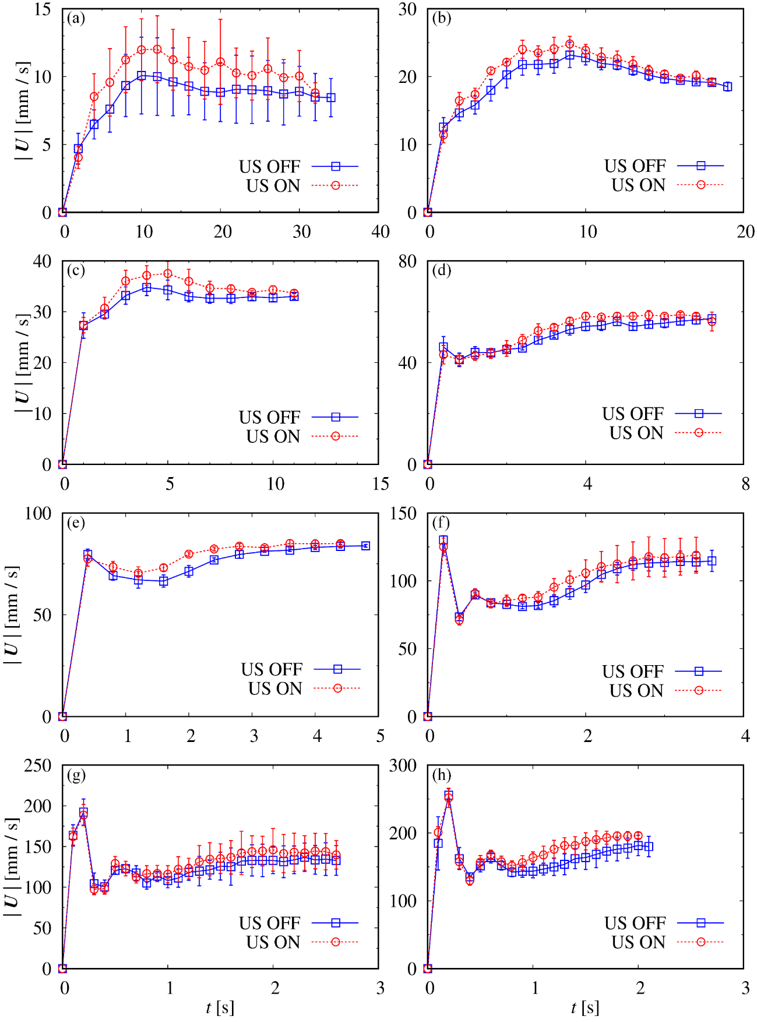
\includegraphics[width=13cm,clip]{X-Appendix/over_shoot/iwamuro-fall.png}
%         \caption{Speed of a falling sphere in diameter of (a) 3 mm, (b) 4 mm, (c) 5 mm, (d) 6 mm, (e) 7 mm, (f) 8 mm, (g) 9 mm, (h) 10 mm in 1.0 wt.\% PAA solution with ultrasound fixed frequency at 27.4 kHz and $\Delta \bar{P} \approx$ 180 kPa\cite{ref:8}.}
%         \label{fig:iwamuro-fall}
%     \end{center}
% \end{figure}

% \begin{figure}[H]
%     \begin{center}
%         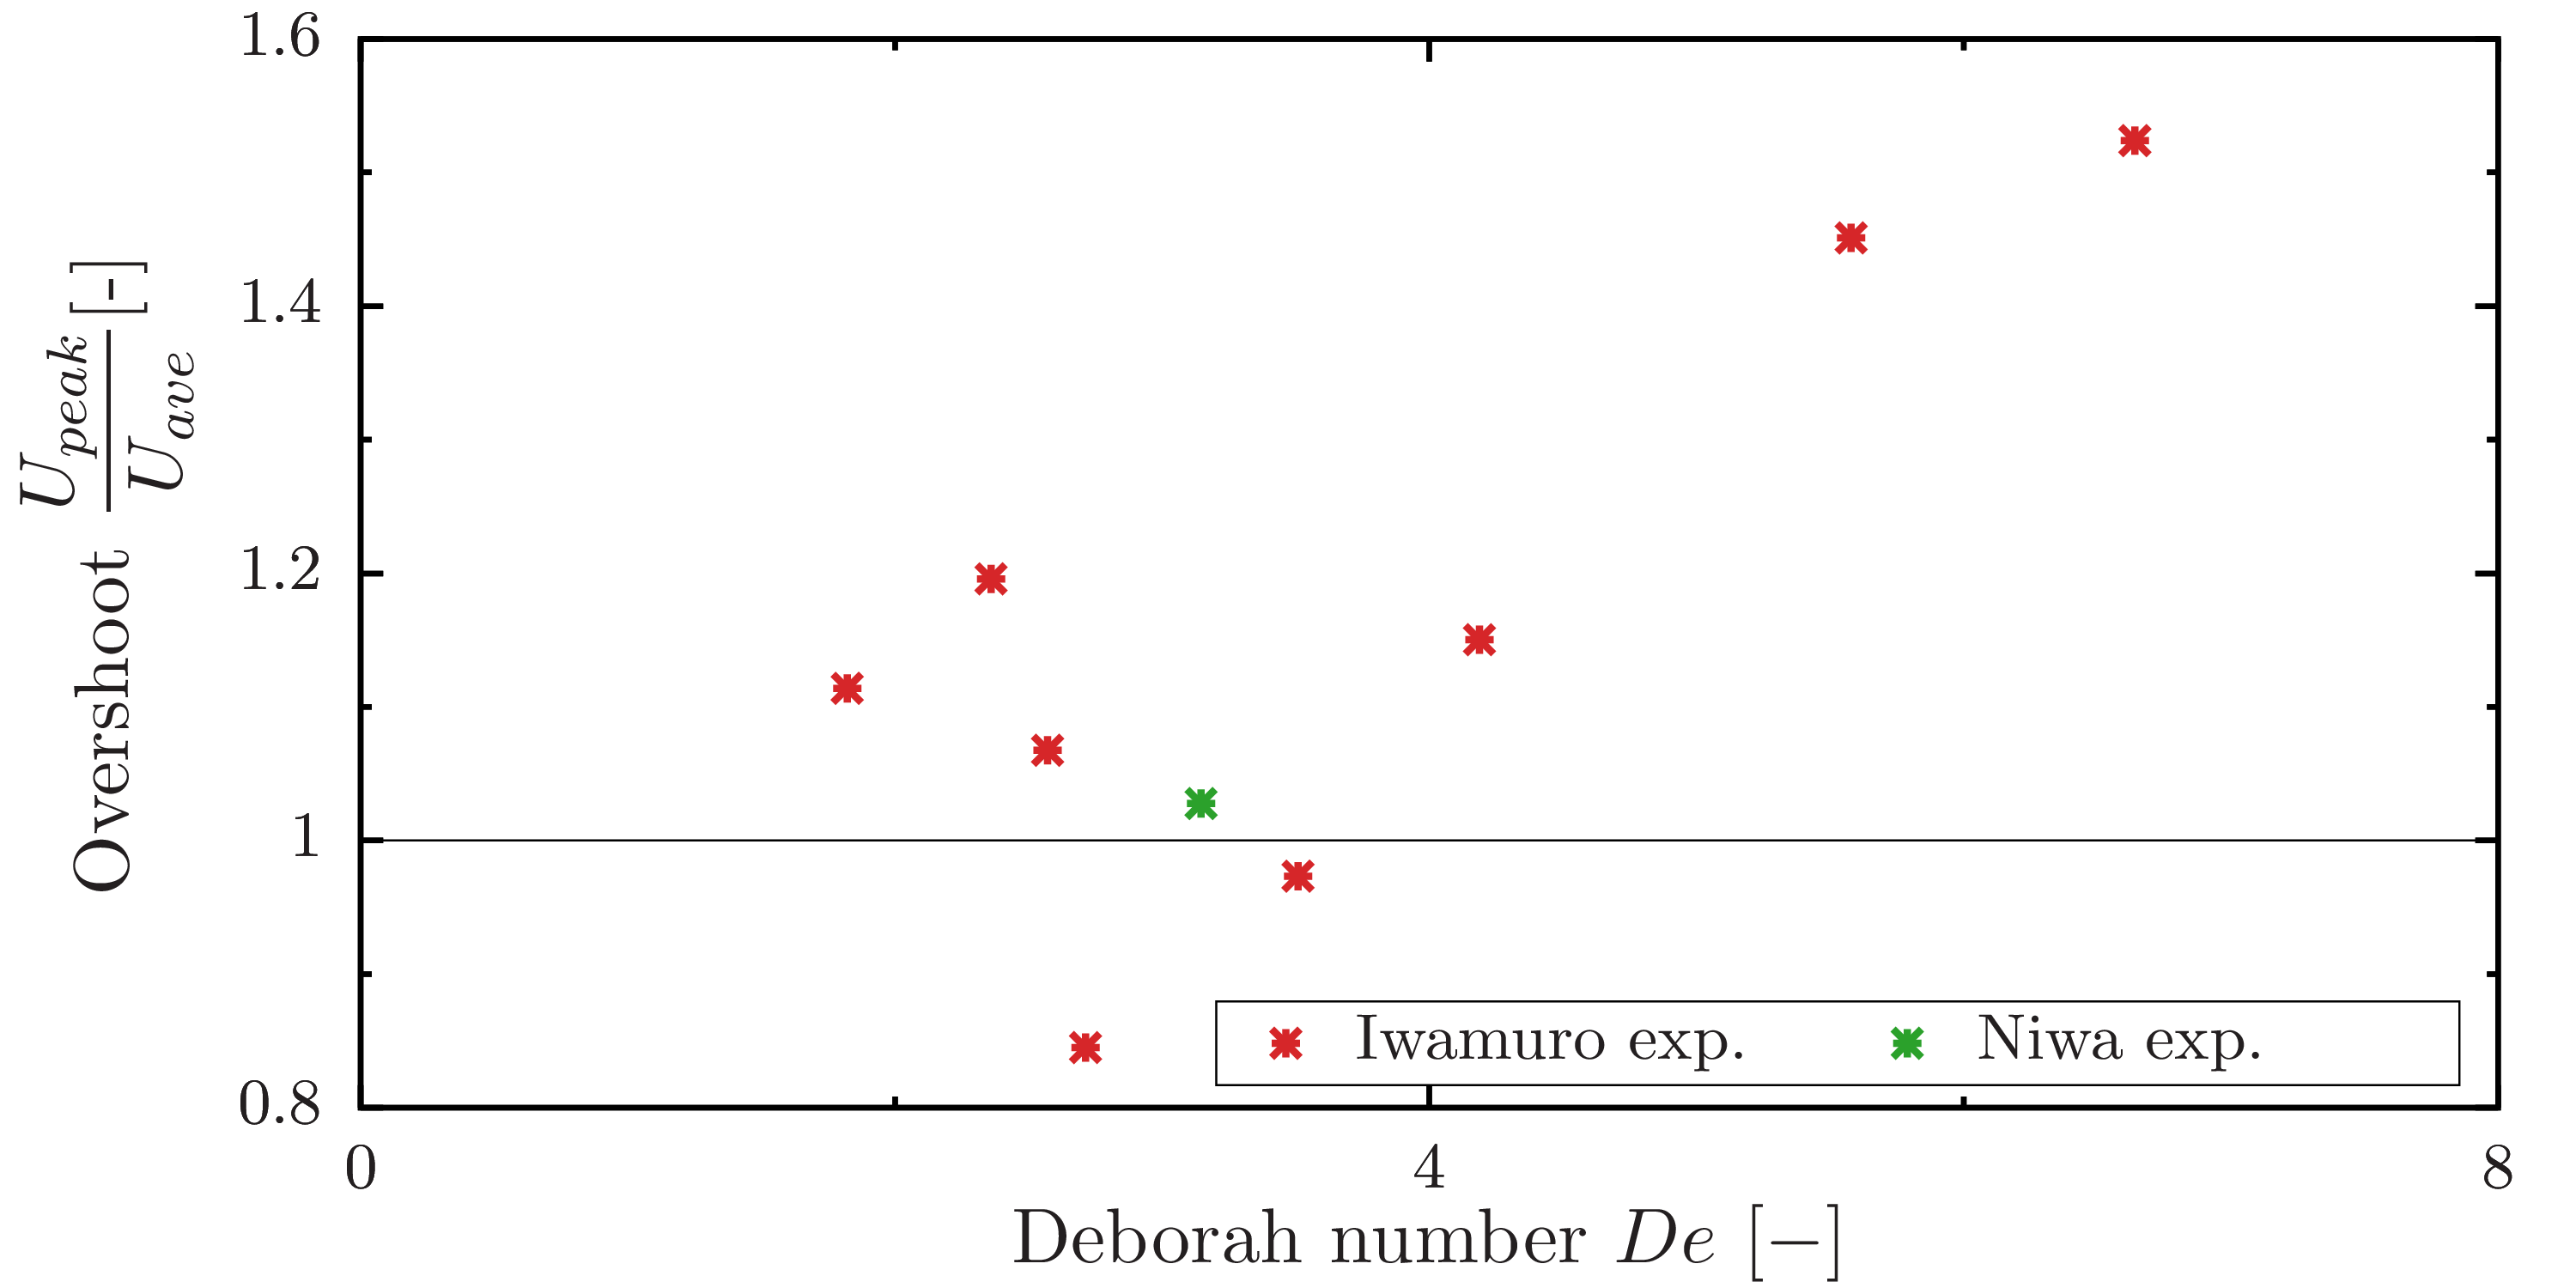
\includegraphics[width=15cm,clip]{5-Results/De-overshoot.png}
%         \caption{Relationship between overshoot $U_{peak}/U_{ave}$ and Deborah number $De$ for falling spheres.}
%         \label{fig:De-overshoot}
%     \end{center}
% \end{figure}

\section{初速による影響に関して}
\label{sec:interval-velocity}
\ref{sec:reexp}章にて,実験装置の改良によってピーク速度が減少し,オーバーシュートが小さくなったことを示した.本節において,電磁石を用いて把持した場合,ピーク速度が大きくなった理由に関して考察を行う.電磁石を用いて球を把持した場合,電磁石へ落下方向に力を与えて落下を開始させている.この時,微小ではあるが落下開始時に初速が存在する.一方で真空ポンプを用いて球を把持した場合,吸着パッドを大気圧にすると球は落下する.この場合,球に力が加わらないため,初速は存在しない.このように初速の有無がオーバーシュートの変化に大きく関与していると考えられる.

初速の有無が与える影響に関して調査するため,真空ポンプを用いて球中心が液面より高さ$H=$5mmとなる地点で把持し,そこから球を落下させた.その結果をFig.\ref{fig:h-5}に示す.縦軸は落下速度,横軸は初速ありの場合は液面に球中心が入ったときを0s,初速なしの場合は落下開始時刻を0sとした時刻である.この条件において,初速は313mm/sとなる.ピーク速度は440mm/sとなり,初速を超えて加速した.これは初速と重力による加速が,粘性抵抗や浮力よりも大きく,弾性は遅れて発生するため,初速を超えて加速したと考えられる.よって,電磁石を用いて球を把持した場合は初速による影響がオーバーシュートとして現れるが,真空ポンプを用いて球を把持した場合は初速が非常に小さいためその影響を受けないということが分かった.

\begin{figure}[H]
    \begin{center}
        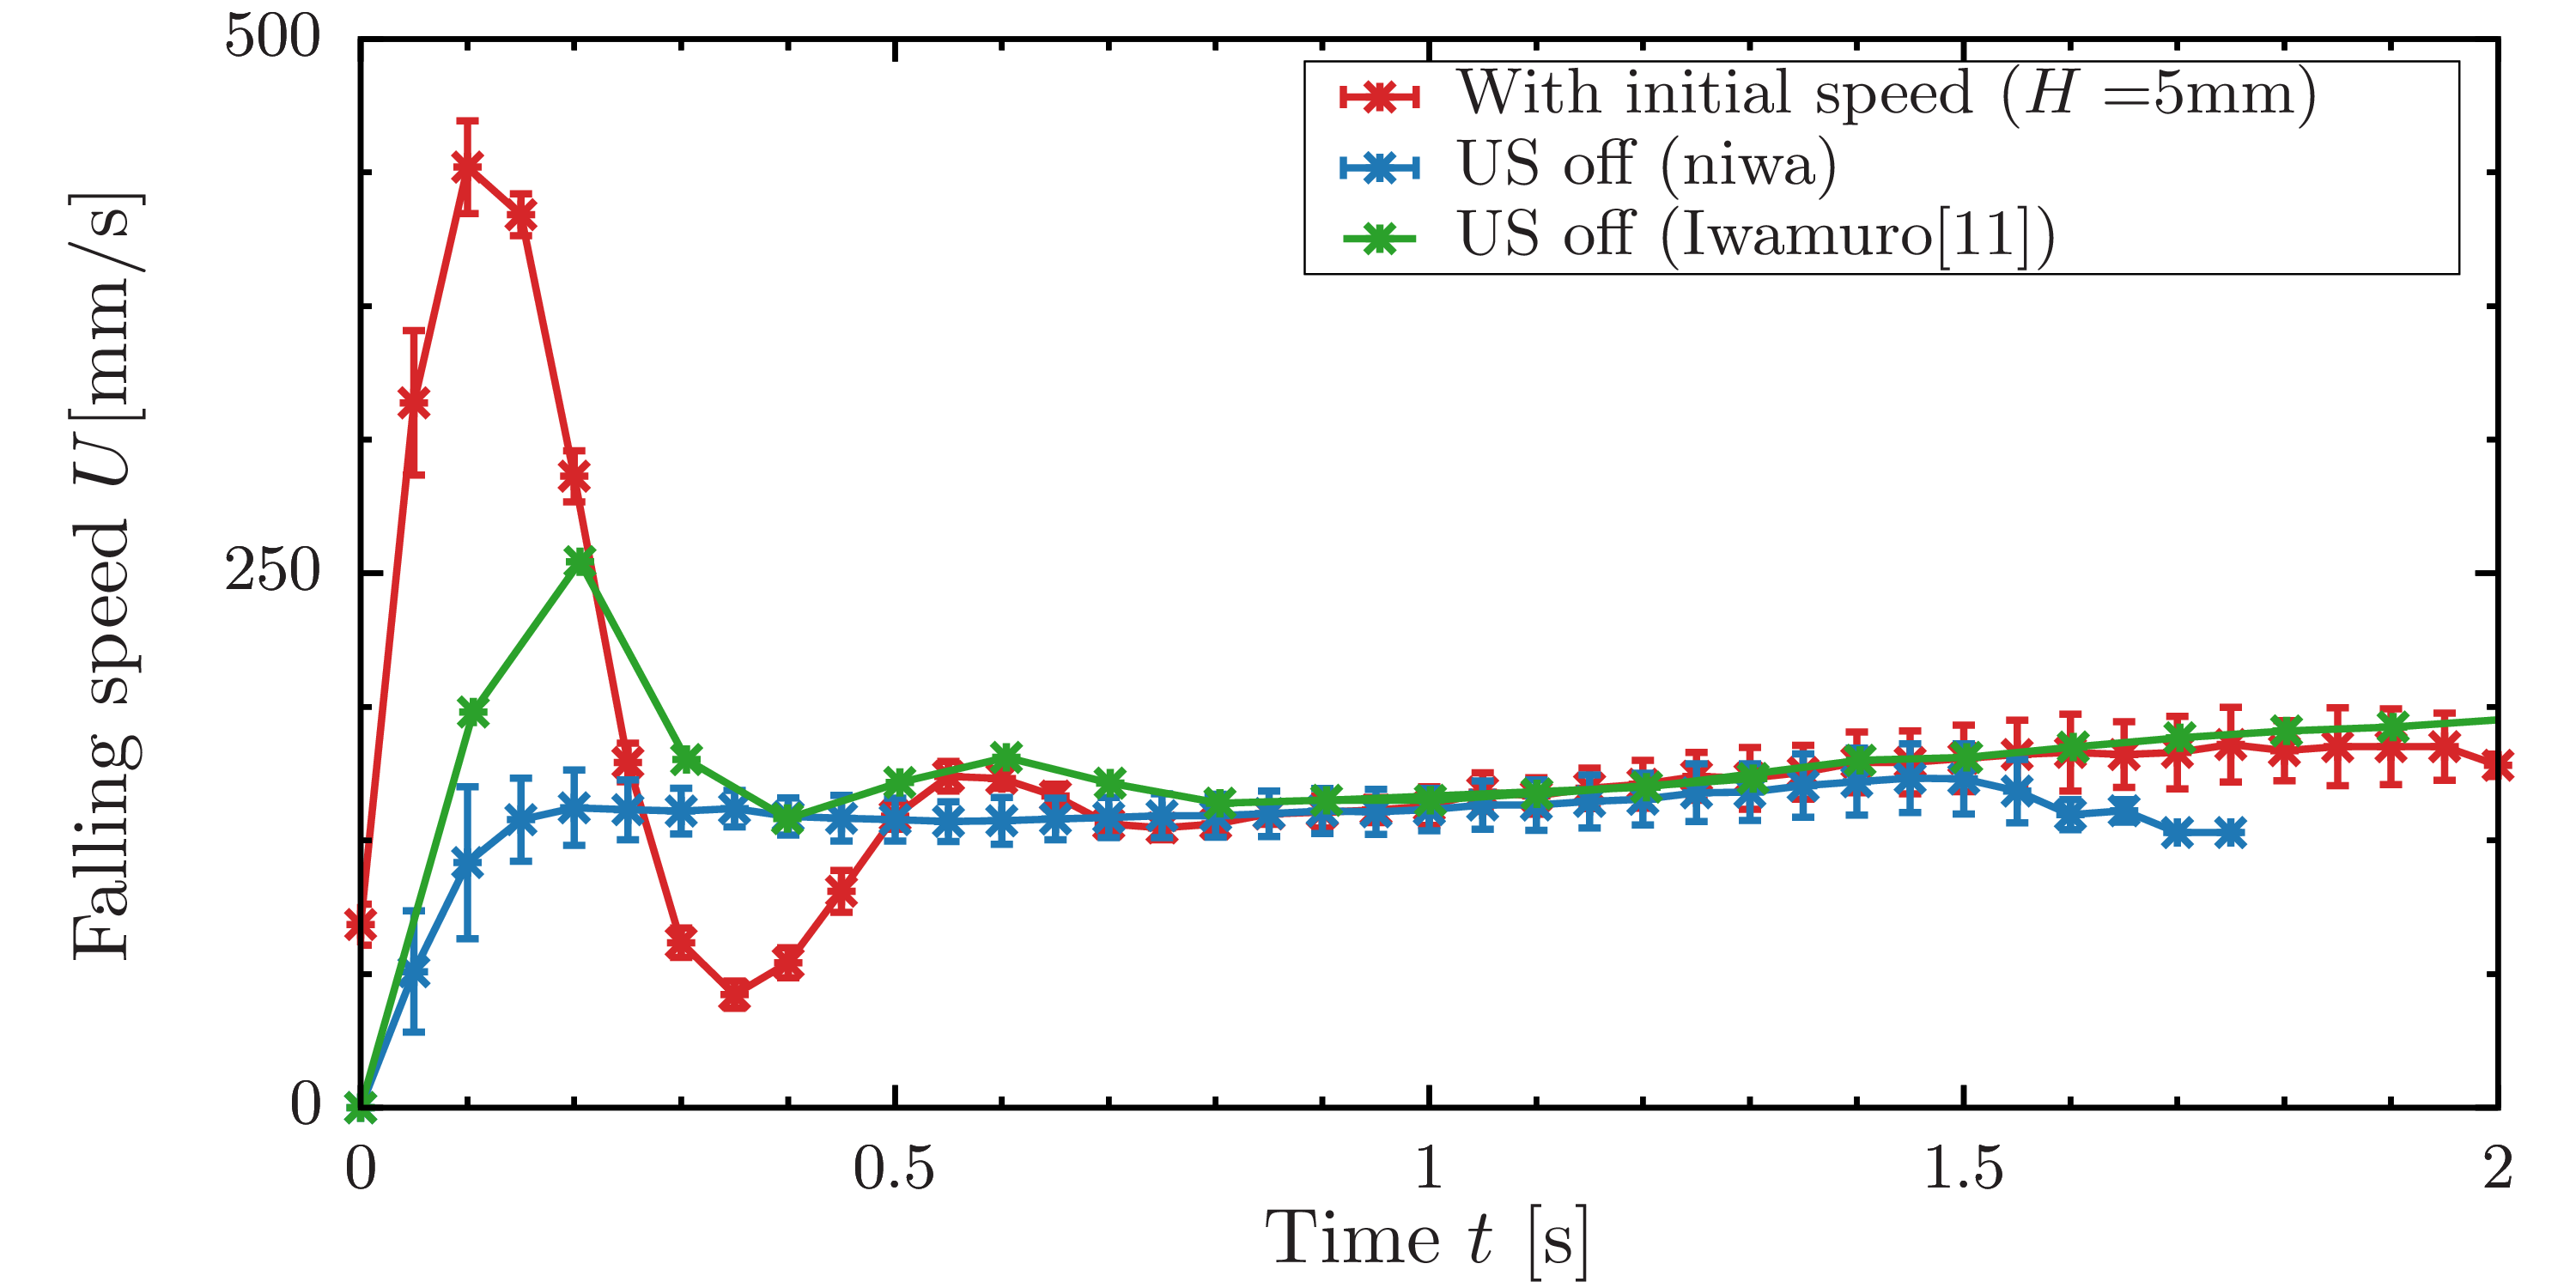
\includegraphics[width=15cm,clip]{X-Appendix/h-5.png}
        \caption{Falling speed of a sphere in 1.0wt.\% PAA solution falling with initial speed.}
        \label{fig:h-5}
    \end{center}
\end{figure}